\section{Evaluation of Filtered Signal}

To demonstrate the effects of low-pass filtering on a
digitally-sampled audio file, we have built an application using
the GNU Radio development framework. In addition to filtering and
playing audio, the application demonstrates the importance of
bandwidth reduction by transmission of the processed audio using
a pair of software-defined radios operating at 903 MHz.

The GNU Radio project \cite{GNU:radio} is an open-source toolkit
supporting the development of software-defined radios. Typically,
application developed by building a flowgraph consisting
of signal-processing components or "blocks" and their interconnects.  

Once the flowgraph is designed, the layout is automatically
converted into a Python program that manages the GNU Radio
scheduler. The scheduler efficiently manages the routing of the
work products to-and-from each block and is not limited by the
speed of the Python interpreter. The signal-processing components
are usually coded in C++ (for performance reasons).

\subsection{Demo Flowgraph Overview}
Our flowgraph is shown in figure \ref{fig:flowgraph} and the
automatically-generated Python code is provided in the Appendix
(Listing \ref{lst:demo}). Note that the interconnected blocks
have multi-colored input and output tabs. The blue tabs show that
the block produces or consumes a complex number, while the orange
tabs indicate the use of simple floating-point values. Input tabs
may only connect to one output tab, but output tabs may connect
to one-or-more input tabs. Every tab must be connected.  

Certain components have no connections.  Primarily these blocks
represent parameter blocks and are used to simplify the layout of
the flowgraph.  The blocks with the labels starting with "QT" 
represent graphical-user interface (GUI) elements that will be 
shown when the application is run.  Our application uses the 
following GUI elements:

\begin{itemize}
	\item Source selection (radio buttons)
	\item Filter selection (radio buttons)
	\item Volume (slider)
	\item Amplitude vs Time (oscilloscope widget)
	\item Amplitude vs Frequency (spectrograph widget)
\end{itemize}

\subsection{Sources}

Three sources are defined for the demo. The first source is
"silence", which is generated by a constant stream of zeros. 

The second source is simply a two-tone signal using 440 Hz (A
above middle C), which is the reference frequency for the
standard musical scale, and 3520 Hz, which is three octaves above
the first tone. When selected in the demo, these two tones
provide a very clear indication of the effects of the 1-kHz
filter.

The third source is a digitally-sampled, CD-quality
snippet from a recording of a performance of "Flight of the
Bumblebee". With an effective bandwidth of 22.05 kHz, this source
is affected by all of the filters. The block is set to
"loop", so that it will run continuously.

A \textit{QT GUI Chooser} drives the source selection block,
allowing the chosen signal to pass to the rest of the flowgraph
while blocking the other two sources.

\subsection{Filter}
Five filter options are defined: 
\begin{itemize}
	\item No filter
	\item 15-kHz filter
	\item 8-kHz filter
	\item 4-kHz filter
	\item 1-kHz filter
\end{itemize}

The filters are implemented using the \textit{FFT Filter} component, which
implements a low-pass filter by taking the Fourier Transform of the
incoming signal, multiplying that by the transfer function
representing the filter, and then performing an inverse-FFT to
generate the output waveform.  The filter parameters are given to 
the block as a sequence of filter taps, as defined above.

As in the source selection, the filter selection is managed by a
QT GUI chooser block driving a selector block.  The output of the 
selector block continues to the rest of the flowgraph.

\subsection{Instrumentation}
In order to visualize the operation of the filters, two GUI elements
are used: an oscilloscope-like widget that charts amplitude versus time,
and a spectrograph-like widget that shows amplitude versus frequency.
When the different filters are chosen, the spectrograph clearly shows
the change in bandwidth of the signal.

\subsection{Output}

Local audio output is provided by an \textit{Audio Sink} block
that drives the default audio device of the computer on which the
program is run. The volume slider controls a multiplier block
that directly affects the amplitude seen by both the and \textit{Audio
Sink} and the radio.

An amplitude-modulation (AM) radio is created in order to
demonstrate a primary benefit of lowpass filtering: radio
transmission bandwidth reduction. The operation of the AM-radio
portion of the flowgraph is beyond the scope of this paper, but
the output drives a software-defined-radio peripheral that
transmits the audio at a center frequency of 903.5 MHz, which is
500 kHz above the base frequency of the radio.

\subsection{Results}

The GNU Radio toolkit provided a very effective platform for
demonstrating the effects of lowpass filtering of different audio
sources. Though not rigorously tested, we observed the behavior
that was expected: the 15-kHz and 8-kHz filters reduced the
bandwidth of the signal, but it was not readily discernible to
our ears. It wasn't until we selected the 4-kHz filter that a
difference was clearly noted.

\begin{figure*}
	\centering
	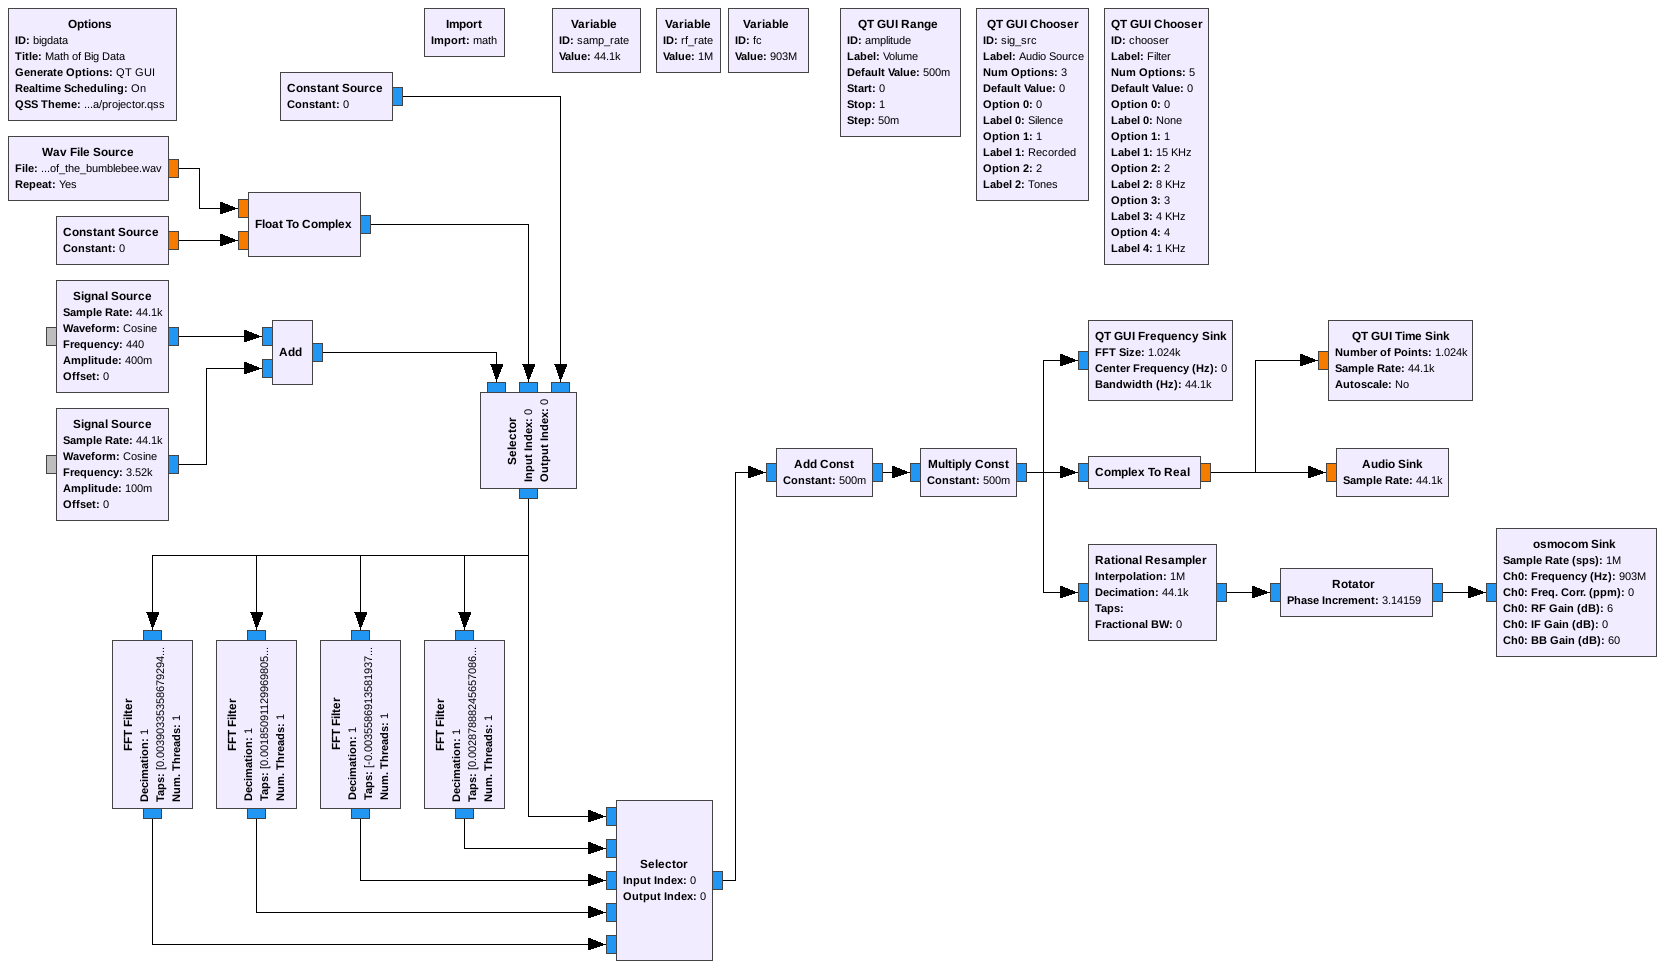
\includegraphics[width=\textwidth]{images/player_grc.png} 
	\caption{Demonstration Application Flowgraph}
	\label{fig:flowgraph}
\end{figure*}    

\begin{figure}
	\centering
	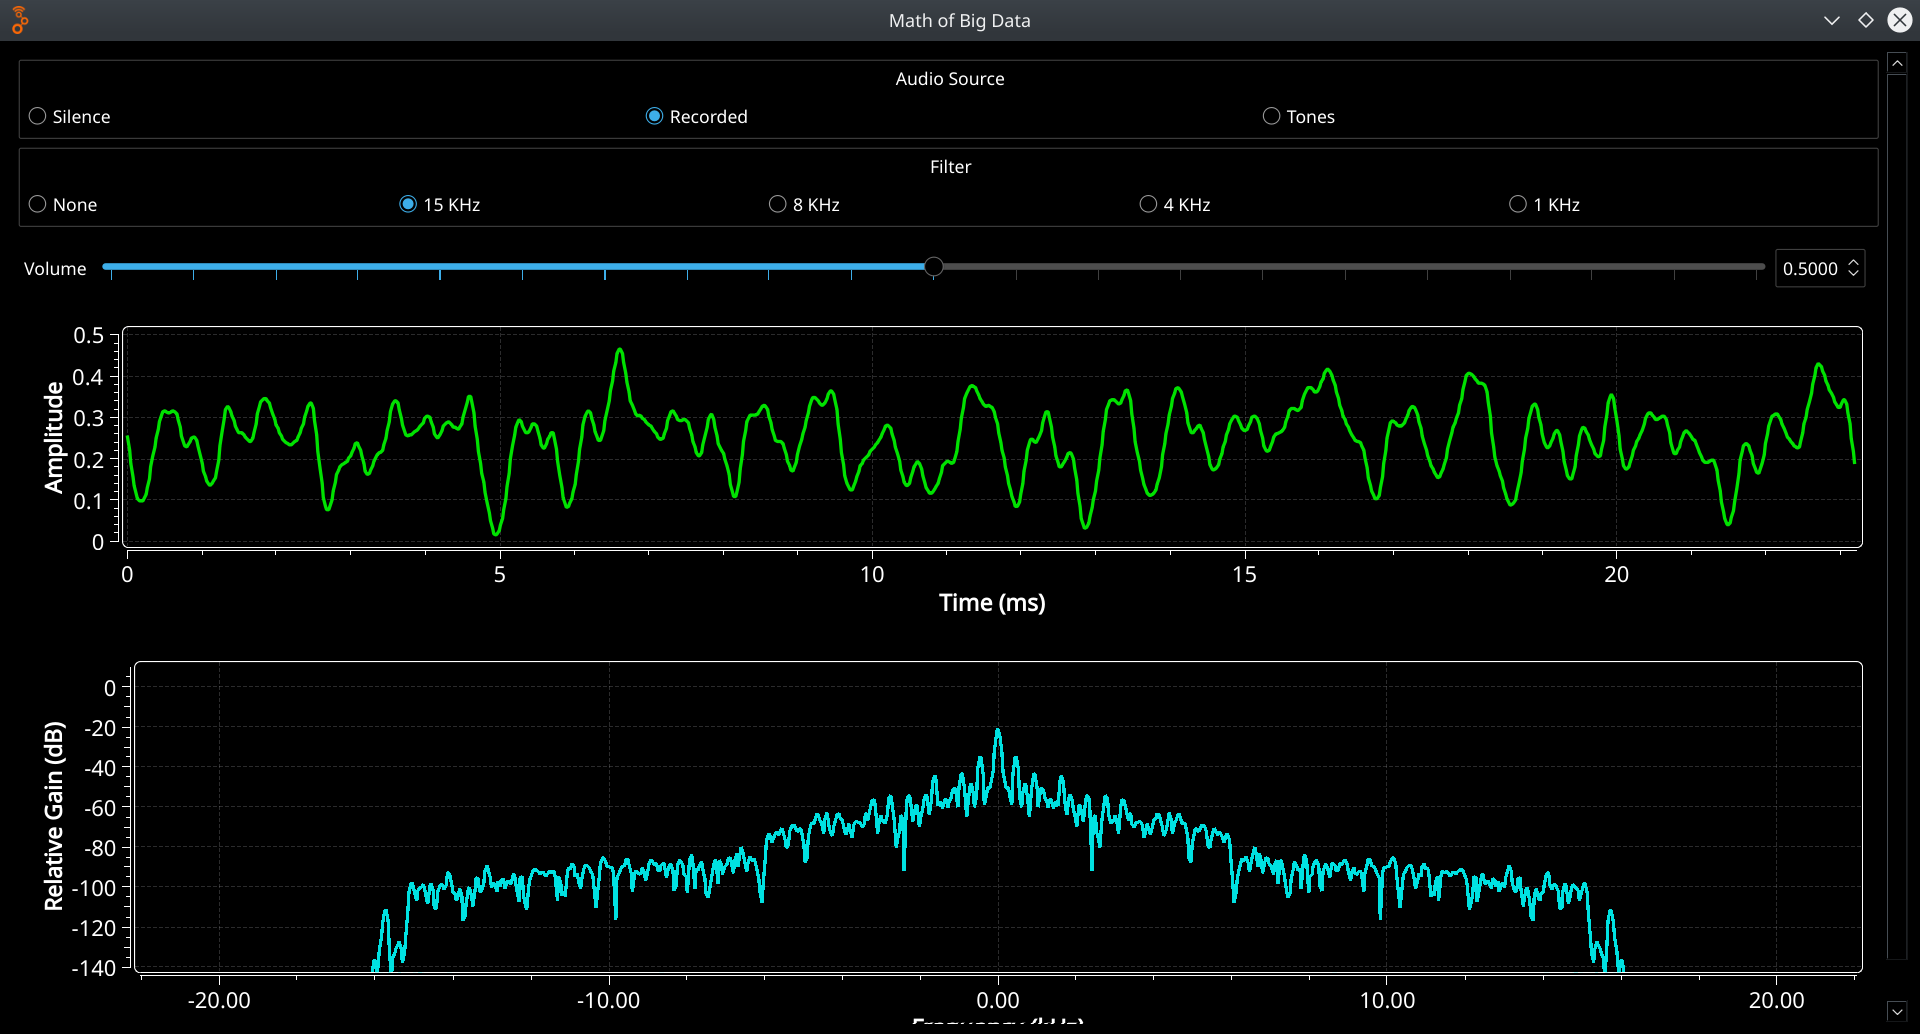
\includegraphics[width=\linewidth]{images/application.png} 
	\caption{Demonstration Application: 15 kHz Filter}
	\label{fig:fifteen}
\end{figure}    

\begin{figure}
	\centering
	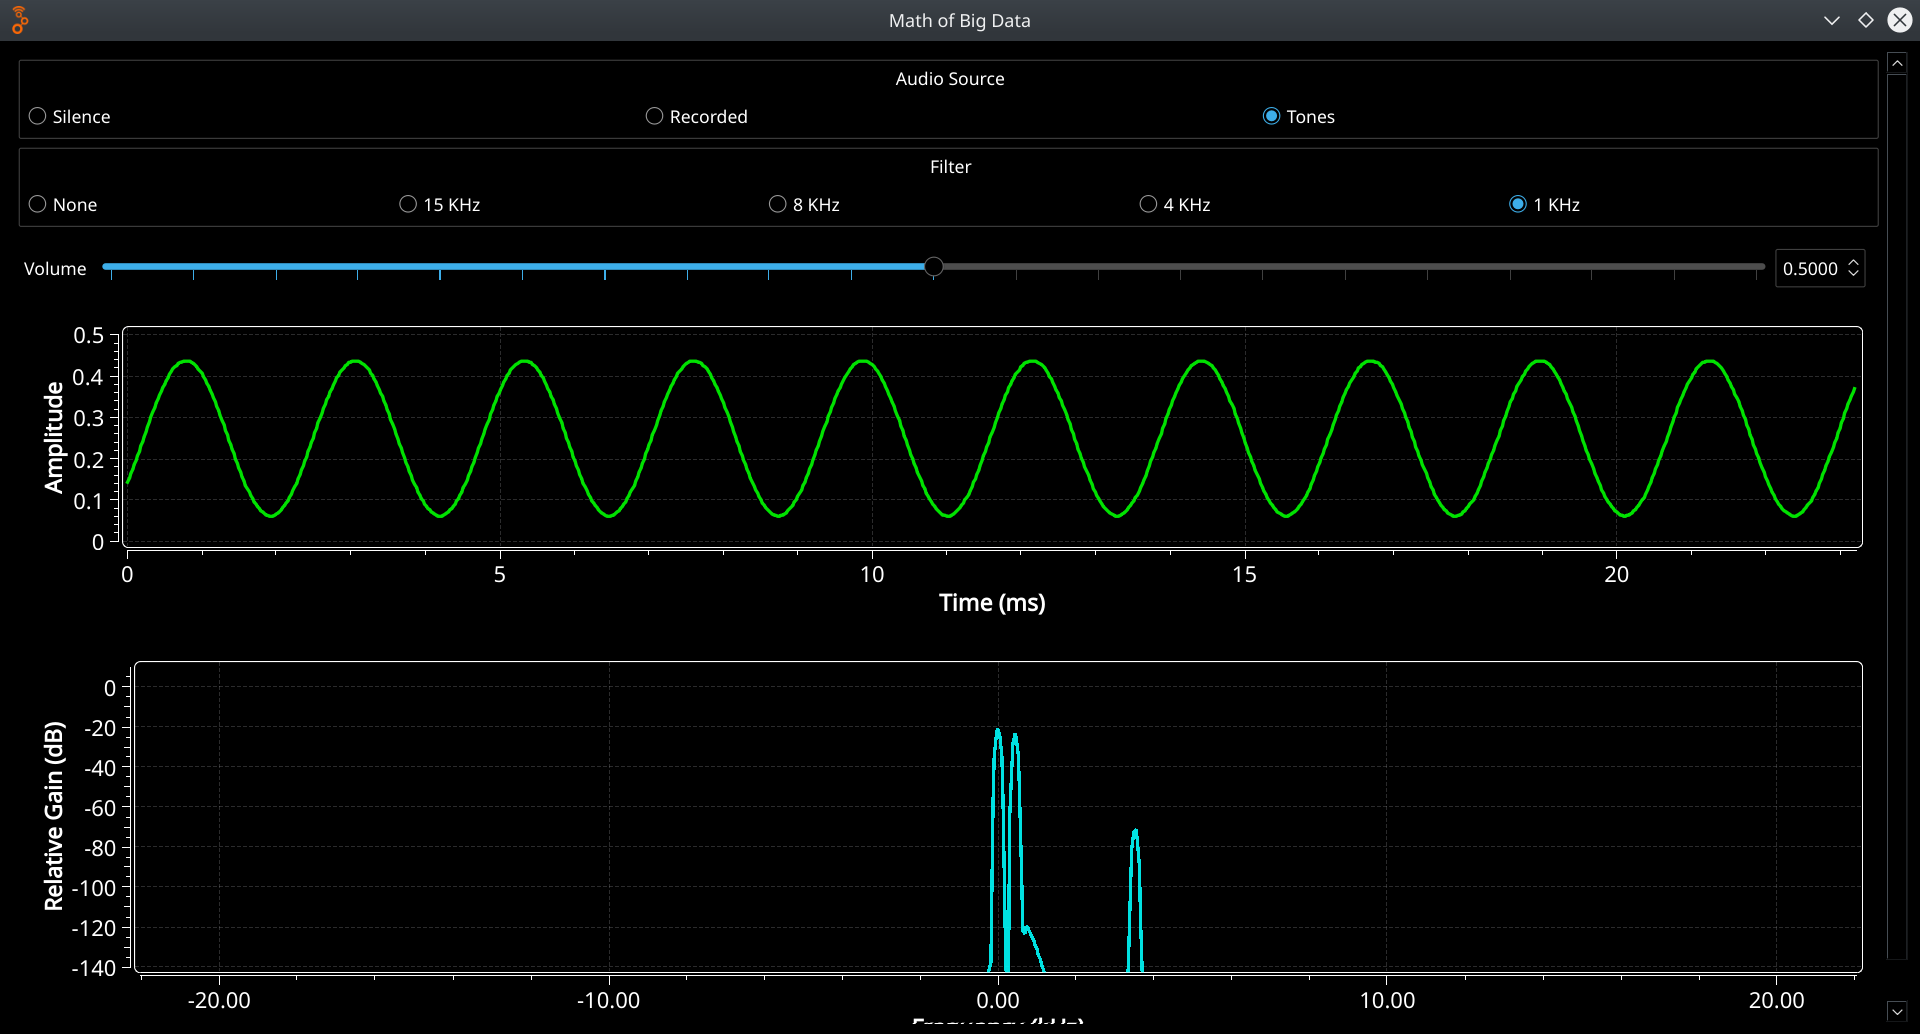
\includegraphics[width=\linewidth]{images/application2.png}
	\caption{Demonstration Application: 1 kHz Filter, Tones}
	\label{fig:tones}
\end{figure}    
